%% Generated by Paper/research/lambda_collapse/make_figure.py -- do not edit by hand.
\definecolor{stepc}{HTML}{0072B2}\definecolor{outc}{HTML}{D55E00}\definecolor{theoc}{HTML}{009E73}\definecolor{midc}{HTML}{CC79A7}
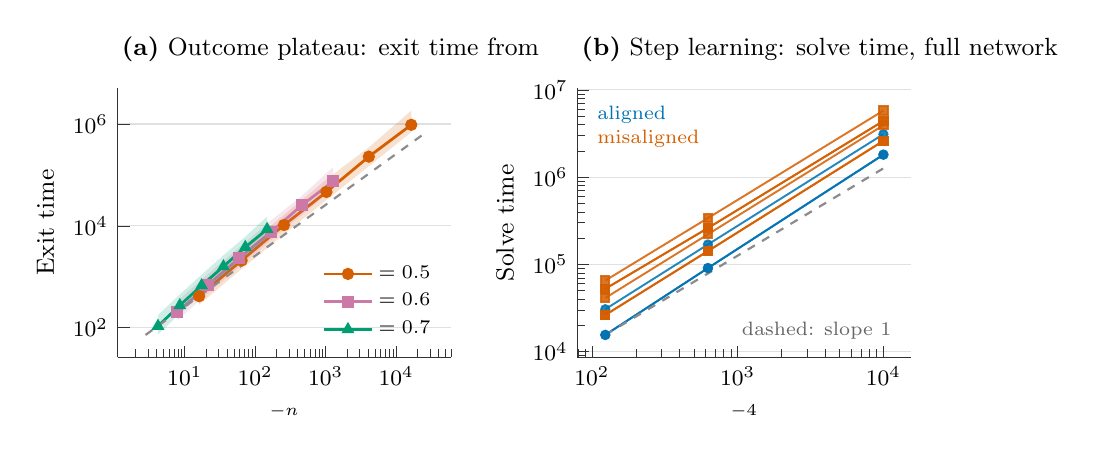
\begin{tikzpicture}
\pgfplotsset{every axis/.style={width=0.48\linewidth, height=5cm, axis line style={black!80}, tick style={black!80},
  tick label style={font=\footnotesize}, label style={font=\small}, title style={font=\small, at={(0,1)}, anchor=south west, xshift=-2pt},
  axis x line*=bottom, axis y line*=left, ymajorgrids, major grid style={black!12}}, every axis plot/.append style={line width=1pt}}
\begin{loglogaxis}[name=pa, title={\textbf{(a)} Outcome plateau: exit time from $\initball$}, xlabel={$\mixrate^{-n}$}, ylabel={Exit time},
  legend style={font=\scriptsize, draw=none, fill=none, at={(0.98,0.03)}, anchor=south east}, legend cell align=left]
  \addplot[draw=none, fill=outc, fill opacity=0.18, forget plot] coordinates {(16,283.012) (64,1413.23) (256,6857.96) (1024,32201.5) (4096,147996) (16384,689161) (16384,1.83425e+06) (4096,347476) (1024,81811.4) (256,16373.4) (64,3385.08) (16,676.199)};
  \addplot[outc, mark=*, mark size=1.7pt] coordinates {(16,413.863) (64,2084) (256,10375.8) (1024,46257.4) (4096,228645) (16384,964510)};
  \addlegendentry{$\mixrate=0.5$}
  \addplot[draw=none, fill=midc, fill opacity=0.18, forget plot] coordinates {(7.71605,136.439) (21.4335,473.075) (59.5374,1580.02) (165.382,5126.31) (459.394,16396.2) (1276.09,53424.4) (1276.09,142473) (459.394,38943.2) (165.382,12616.4) (59.5374,3785.17) (21.4335,1132.53) (7.71605,325.944)};
  \addplot[midc, mark=square*, mark size=1.7pt] coordinates {(7.71605,198.99) (21.4335,691.557) (59.5374,2333.01) (165.382,7444.27) (459.394,25414.7) (1276.09,75030.9)};
  \addlegendentry{$\mixrate=0.6$}
  \addplot[draw=none, fill=theoc, fill opacity=0.18, forget plot] coordinates {(4.16493,73.6358) (8.49986,187.581) (17.3467,459.286) (35.4013,1092.83) (72.2476,2551.12) (147.444,5945.42) (147.444,15264.5) (72.2476,6115.4) (35.4013,2639.29) (17.3467,1100.71) (8.49986,448.967) (4.16493,175.9)};
  \addplot[theoc, mark=triangle*, mark size=1.7pt] coordinates {(4.16493,107.269) (8.49986,273.487) (17.3467,671.624) (35.4013,1590.59) (72.2476,3811.26) (147.444,8579.4)};
  \addlegendentry{$\mixrate=0.7$}
  \addplot[black!45, dashed, line width=0.8pt, forget plot] coordinates {(2.77662,71.8213) (24576,635694)};
\end{loglogaxis}
\begin{loglogaxis}[name=pb, at={(pa.east)}, anchor=west, xshift=1.6cm, title={\textbf{(b)} Step learning: solve time, full network},
  xlabel={$\initscale^{-4}$}, ylabel={Solve time}]
  \addplot[stepc, mark=*, mark size=1.5pt, line width=0.7pt, opacity=0.85] coordinates {(123.457,30650.7) (625,169041) (10000,3.1062e+06)};
  \addplot[stepc, mark=*, mark size=1.5pt, line width=0.7pt, opacity=0.85] coordinates {(123.457,15553.8) (625,90722.3) (10000,1.8088e+06)};
  \addplot[stepc, mark=*, mark size=1.5pt, line width=0.7pt, opacity=0.85] coordinates {(123.457,15553.8) (625,90722.3) (10000,1.8088e+06)};
  \addplot[outc, mark=square*, mark size=1.5pt, line width=0.7pt, opacity=0.85] coordinates {(123.457,41234.3) (625,221303) (10000,3.93086e+06)};
  \addplot[outc, mark=square*, mark size=1.5pt, line width=0.7pt, opacity=0.85] coordinates {(123.457,26321.5) (625,142089) (10000,2.60491e+06)};
  \addplot[outc, mark=square*, mark size=1.5pt, line width=0.7pt, opacity=0.85] coordinates {(123.457,26321.5) (625,142089) (10000,2.60491e+06)};
  \addplot[outc, mark=square*, mark size=1.5pt, line width=0.7pt, opacity=0.85] coordinates {(123.457,65306.9) (625,339230) (10000,5.78317e+06)};
  \addplot[outc, mark=square*, mark size=1.5pt, line width=0.7pt, opacity=0.85] coordinates {(123.457,52523.9) (625,260828) (10000,4.40218e+06)};
  \addplot[outc, mark=square*, mark size=1.5pt, line width=0.7pt, opacity=0.85] coordinates {(123.457,52523.9) (625,260828) (10000,4.40218e+06)};
  \addplot[black!45, dashed, line width=0.8pt] coordinates {(123.457,15553.8) (10000,1.25985e+06)};
  \node[anchor=north west, font=\scriptsize, text=stepc] at (rel axis cs:0.03,0.97) {aligned};
  \node[anchor=north west, font=\scriptsize, text=outc] at (rel axis cs:0.03,0.88) {misaligned};
  \node[anchor=south east, font=\scriptsize, text=black!60] at (rel axis cs:0.97,0.03) {dashed: slope $1$};
\end{loglogaxis}
\end{tikzpicture}
